% oss-plantilla: oss-2026.10
% Preámbulo corporativo fijo. No editar en sd-NN.tex: exportar_latex.py verificar lo compara byte a byte.
% Para cambiar el formato, editar esta plantilla u oss.sty y subir la versión de la primera línea.
\PassOptionsToPackage{unicode}{hyperref}
\PassOptionsToPackage{hyphens}{url}
\documentclass[11pt]{article}
\usepackage{amsmath,amssymb}
\usepackage{fontspec}
\defaultfontfeatures{Ligatures=TeX,Scale=MatchLowercase}
\setmainfont{DejaVu Sans}
\setsansfont{DejaVu Sans}
\setmonofont{DejaVu Sans Mono}
\usepackage[letterpaper,margin=20mm]{geometry}
\usepackage{microtype}
\usepackage{parskip}
\usepackage{xcolor}
\usepackage{longtable,booktabs,array}
\usepackage{calc}
\usepackage{etoolbox}
\makeatletter
\patchcmd\longtable{\par}{\if@noskipsec\mbox{}\fi\par}{}{}
\makeatother
\usepackage{footnotehyper}
\makesavenoteenv{longtable}
\usepackage{graphicx}
\makeatletter
\newsavebox\pandoc@box
\newcommand*\pandocbounded[1]{%
  \sbox\pandoc@box{#1}%
  \Gscale@div\@tempa{\textheight}{\dimexpr\ht\pandoc@box+\dp\pandoc@box\relax}%
  \Gscale@div\@tempb{\linewidth}{\wd\pandoc@box}%
  \ifdim\@tempb\p@<\@tempa\p@\let\@tempa\@tempb\fi
  \ifdim\@tempa\p@<\p@\scalebox{\@tempa}{\usebox\pandoc@box}%
  \else\usebox{\pandoc@box}%
  \fi}
\def\maxwidth{\ifdim\Gin@nat@width>\linewidth\linewidth\else\Gin@nat@width\fi}
\def\maxheight{\ifdim\Gin@nat@height>\textheight\textheight\else\Gin@nat@height\fi}
\makeatother
\setkeys{Gin}{width=\maxwidth,height=\maxheight,keepaspectratio}
\makeatletter
\def\fps@figure{htbp}
\makeatother
\usepackage[normalem]{ulem}
\providecommand{\st}[1]{\sout{#1}}
\usepackage{fancyvrb}
\setlength{\emergencystretch}{3em}
\providecommand{\tightlist}{%
  \setlength{\itemsep}{0pt}\setlength{\parskip}{0pt}}
\providecommand{\passthrough}[1]{#1}
\setcounter{secnumdepth}{-\maxdimen}
\usepackage[bidi=default]{babel}
\babelprovide[main,import]{spanish}
\let\LanguageShortHands\languageshorthands
\def\languageshorthands#1{}
\usepackage{bookmark}
\usepackage{xurl}
\urlstyle{same}
\hypersetup{pdflang={es-CL},pdfcreator={Only Simple Solutions - exportar_latex.py}}
\usepackage{oss}
\begin{document}

\ossCover{Resumen Ejecutivo, comprensión del problema y de la necesidad}{Subdocumento 2}
\tableofcontents
\clearpage

\hypertarget{resumen-ejecutivo-del-problema}{%
\section{2.1 Resumen Ejecutivo del problema}\label{resumen-ejecutivo-del-problema}}

\hypertarget{comprensiuxf3n-del-problema-y-la-necesidad}{%
\subsection{COMPRENSIÓN DEL PROBLEMA Y LA NECESIDAD}\label{comprensiuxf3n-del-problema-y-la-necesidad}}

Multitiendas Ancoa S.A. es una cadena de tiendas por departamento chilena, sociedad anónima cerrada, en operación desde 1972, con ingresos consolidados de \textbf{\$474.000 millones de pesos}, esta se rige bajo la Ley del consumidor N°19.496 (Congreso Nacional de Chile, 2021) . Simultáneamente, se consolida como un emisor de crédito fiscalizado, en donde el negocio financiero se desarrolla a través de una filial emisora de tarjeta de casa comercial, sujeta a la fiscalización de la CMF (Información de Supervisados, s. f.). Ambos dominios están sujetos a la nueva Ley de datos personales. N°21.719 (Congreso Nacional de Chile, 2026) .

Actualmente, Ancoa enfrenta una brecha entre lo que promete a sus clientes, lo que sus registros permiten conocer y lo que puede acreditar después, la compañía realiza cuatro promesas operacionales, las cuales consisten en que el producto existe, que el precio cobrado coincide con el exhibido, que la entrega llegará en la fecha informada y que las condiciones del crédito son las entregadas y aceptadas. Estas cuatro promesas dependen de información que está fragmentada, no está sincronizada y es no recuperable.

Esto queda expuesto en tres hechos concretos en donde \textbf{2.840} pedidos fueron cancelados por falta de existencia durante un evento de \textbf{104.000} pedidos, discrepancias de precios en el \textbf{11\%} de 120 productos revisados en cuatro tiendas y \textbf{1.240} repactaciones de 2025 que no tenían evidencia recuperable del consentimiento. En paralelo, el cumplimiento de la fecha de entrega es del \textbf{81\%}, en donde existen nueve plataformas conectadas por catorce interfaces cuyo mapa completo no está disponible y la separación de los datos entre el retail y la filial emisora es parcial y no documentada.

El problema afecta a todos los asociados a Ancoa, es decir, cliente, titulares de tarjeta, vendedores, cajeros, jefaturas de tienda, logística, canales digitales, comercial, la filial financiera, TI, vendedores de marketplace, proveedores y autoridades fiscalizadoras. En cuanto a su resolución futura deberá reconocer que Ancoa opera dos negocios ante una misma persona, retail y crédito que comparten marca y puntos de contacto, pero no pueden compartir libremente datos ni obligaciones.

Sumando a esto, se agregan tres situaciones futuras que deben ser abordadas obligatoriamente por en el proyecto. Por una parte, está la migración de la cartera de \textbf{620.000} clientes con saldo desde la plataforma antigua hacía la nueva, proceso que deberá realizarse sin pérdida de información, interrupción del servicio ni discrepancias en los saldos. Por otra parte, está el término en el año 2029 del soporte proporcionado por el fabricante de la plataforma de originación y cobranza de créditos actualmente en operación desde 2011. Finalmente, tenemos el vencimiento, en el año \textbf{2029} del último hito del plan de remediación instruido por la autoridad fiscalizadora. Si estos inconvenientes no son resueltos, Ancoa podría enfrentar interrupciones en la operación financiera, inconsistencias en las cuentas de sus clientes, dependencia de una plataforma sin soporte e incumplimientos ante la autoridad competente.

\hypertarget{comprensiuxf3n-del-problema-y-de-la-necesidad}{%
\section{2.2 Comprensión del problema y de la necesidad}\label{comprensiuxf3n-del-problema-y-de-la-necesidad}}

Esta sección profundiza en las condiciones propias de la industria y de la operación que explican el problema presentado anteriormente. Para ello, se consideran las características del modelo omnicanal, la convivencia entre el retail y el negocio financiero, el marco regulatorio aplicable y la estacionalidad del comercio, sin abordar todavía el dimensionamiento detallado del problema ni las decisiones asociadas a su solución.

\hypertarget{contexto-de-la-industria}{%
\subsection{Contexto de la industria}\label{contexto-de-la-industria}}

La operación de Multitiendas Ancoa S.A. combina una red tiendas físicas con un alcance a nivel nacional con canales digitales y un marketplace de terceros. A esta actividad se suma el negocio financiero, desarrollado mediante una filial emisora de tarjeta de casa comercial. De esta forma, Ancoa participa simultáneamente en la industria del comercio minorista y en el sector financiero, actividades que se relacionan directamente en el punto de venta y frente a un mismo cliente.

La compañía mantiene 22 tiendas distribuidas en 11 regiones, de las cuales 14 funcionan dentro de centros comerciales y ocho corresponden a tiendas con acceso a la calle. En conjunto, estas instalaciones suman 96.000 m² de superficie de venta y presentan condiciones operativas distintas entre sí, desde la tienda insignia ubicada en Santiago hasta establecimientos más pequeños y aislados, como el ubicado en Coyhaique, que presentan restricciones de conectividad y abastecimiento.

El funcionamiento físico de la tienda se complementa con el canal en línea y el marketplace. Su canal digital representa un 19\% de las ventas y procesa aproximadamente 1,9 millones de pedidos al año. A la vez, cerca del 71\% de las referencias del catálogo corresponden a vendedores externos del marketplace, mientras que el 29\% restante corresponde a referencias del catálogo propio. Esto implica que Ancoa no se limita al modelo tradicional de compra y venta en el local, sino que debe coordinar productos, inventario y atención al cliente entre canales propios y de terceros.

Como referencia del sector, la Cámara de Comercio de Santiago estimó que durante 2025 el comercio electrónico representó un 12,6\% de las ventas del comercio minorista en Chile y un 16,1\% en el caso de las tiendas por departamento. Además, las ventas online crecieron un 11,6\% nominal durante ese año. En este contexto, la participación digital de Ancoa, equivalente al 19\% de sus ventas, se encuentra por sobre la referencia informada para las tiendas por departamento y confirma que el canal digital tiene un peso relevante dentro de su operación (Cámara de Comercio de Santiago {[}CCS{]}, 2026a).

Las tiendas tampoco se limitan a participar en la venta presencial. Un 41\% de los pedidos en línea son retirados en tienda, y también despachan a un 17\% de estos. Por esto parte de la infraestructura y del personal de sala participa directamente en el cumplimiento de los pedidos digitales. Las mesas de atención también realizan los cambios, devoluciones y reciben los reclamos de distintos canales. Es por esto que la tienda física, el canal digital y el marketplace funcionan mediante procesos que ocupan, en cierto grado, la misma infraestructura y personal.

\hypertarget{particularidades-operacionales}{%
\subsubsection{Particularidades operacionales}\label{particularidades-operacionales}}

La principal particularidad del funcionamiento de Ancoa es que las actividades de los sectores de retail y financiero coinciden en el mismo entorno operacional. El negocio financiero funciona mediante una filial distinta, pero comparte con el retail la marca, el cliente y parte de los puntos de atención. Durante una visita a la tienda, la misma persona puede comprar un producto, pagar con su tarjeta propia y realizar gestiones relacionadas al crédito. Es por esta convivencia que procesos de ambos negocios se pueden realizar frente al mismo cliente, y en algunos casos por el mismo personal.

A esto se suma la naturaleza fragmentada del entorno tecnológico. El negocio funciona gracias a nueve plataformas de seis proveedores, conectadas mediante catorce interfaces punto a punto a lo largo de quince años. Varias de estas plataformas comparten información mediante procesos nocturnos, y Ancoa no cuenta con un mapa completo de todas las conexiones entre sistemas. Esto implica que la información utilizada por el negocio puede encontrarse distribuida entre distintas plataformas, y no actualizarse al mismo tiempo.

Otra condición sensible es la relación entre el retail y la filial financiera. Ambos comparten centros de datos, red y equipos de tecnologías de la información, mientras que su separación lógica está implementada de manera parcial, y no completamente documentada. Por lo tanto, aunque comparte la infraestructura tecnológica, la información de ambos negocios no puede tratarse sin hacer la distinción necesaria.

La fuerza laboral también condiciona la forma en que se ejecutan los procesos. La compañía cuenta con 3.820 vendedores de piso y cajeros, cuya remuneración posee un componente variable asociado a comisiones y cuya rotación anual alcanza el 62\%. La comisión aumenta cuando una venta se paga mediante la tarjeta propia, por lo que el tiempo requerido para completar los procesos comerciales y financieros forma parte de las condiciones habituales de trabajo del vendedor.

En las salas de venta trabajan aproximadamente 1.100 repositores que están contratados por proveedores externos, y no tienen relación laboral directa con Ancoa. A esto se suma que los vendedores comparten 640 terminales móviles para consultar la existencia de productos, las cuales están distribuidas de forma desigual entre las tiendas. Estas condiciones deben considerarse para comprender una operación en la que interactúan personal propio, personal externo, equipos compartidos y procesos presenciales y digitales.

\hypertarget{particularidades-regulatorias}{%
\subsubsection{Particularidades regulatorias}\label{particularidades-regulatorias}}

La coexistencia de ambos dominios hace que Ancoa se rige por regímenes jurídicos de distinta naturaleza.

En lo que respecta al dominio del retail, materia de protección al consumidor, la Ley N.º 19.496 establece obligaciones relacionadas con la información proporcionada al cliente y los precios de los bienes y servicios. Su artículo 30 exige que el precio sea informado de forma claramente visible antes de perfeccionarse el acto de consumo y contempla también la oferta de productos realizada mediante sitios de Internet (Ley N.º 19.496, 1997). Esto es relevante en una operación donde un mismo producto puede tener un precio registrado centralmente, uno publicado en el canal digital y una etiqueta física exhibida en tienda.

Por otro lado y dentro del mismo dominio, el canal digital está sujeto al decreto N°6 del 2021, Reglamento del comercio electrónico. Esta normativa establece los deberes de información en las ventas realizadas mediante medios digitales y distingue las obligaciones de los vendedores y operadores de las plataformas electrónicas. (Decreto N.º 6, 2021)

En particular, el reglamento exige informar aspectos como el costo total de la compra, la inexistencia de stock, los plazos de despacho o retiro y los canales de contacto para consultas, cambios o devoluciones. Estas obligaciones resultan especialmente relevantes en operaciones que combinan comercio electrónico, retiro en tienda y marketplace (Servicio Nacional del Consumidor {[}SERNAC{]}, 2022).

La filial financiera se encuentra bajo un marco distinto para cada una de sus áreas. Por un lado los emisores de tarjetas de crédito no bancarias forman parte de las entidades reguladas y supervisadas por la Comisión para el Mercado Financiero, mientras que las operaciones de crédito de dinero se encuentran reguladas por la Ley N.º 18.010 (Ley N.º 18.010, 1981). Por lo que, procesos como la originación, modificación de condiciones, repactación y cobranza poseen exigencias distintas a las de una venta de retail.

La diferencia entre ambos dominios también trae consigo responsabilidades distintas respecto al tratamiento de la información. La empresa tiene interés en utilizar los antecedentes de sus clientes del dominio de retail para análisis y campañas, mientras que la información del dominio de la filial ha sido utilizada para finalidades asociadas al crédito. El cruce de información entre ambos ámbitos requiere determinar previamente qué datos pueden utilizarse, con qué finalidad y bajo qué fundamento.

Durante el horizonte del proyecto también deberá considerarse la Ley N.º 21.719, que regula la protección y el tratamiento de los datos personales y crea la Agencia de Protección de Datos Personales. La norma fue publicada el 13 de diciembre de 2024 y su entrada en vigencia está fijada para el 1 de diciembre de 2026 (Ley N.º 21.719, 2024). Esto es especialmente relevante por la cantidad y diversidad de información de clientes procesada entre los canales comerciales y el negocio financiero.

Por estas razones, una interacción con un cliente está sujeta a restricciones distintas dependiendo del ámbito del negocio con el que esté interactuando. La particularidad regulatoria de Ancoa radica en que estas actividades están estrechamente relacionadas en la operación diaria, aunque no se encuentran sometidas a un único régimen jurídico.

\hypertarget{particularidades-estacionales}{%
\subsubsection{Particularidades estacionales}\label{particularidades-estacionales}}

Durante el transcurso del año hay períodos en que la demanda aumenta a niveles considerablemente distintos del régimen normal. Entre el 1 de noviembre y el 6 de enero se desarrolla la campaña de navidad, y la posterior liquidación de enero, lo que corresponde al nivel de demanda más alto de las ventas. Durante esta etapa, la dotación aumenta desde aproximadamente 6.400 hasta 8.300 trabajadores mediante la incorporación de cerca de 1.900 personas de temporada.

También existen otros períodos de mayor actividad durante el año. La temporada de vuelta a clases se extiende aproximadamente desde la última semana de enero hasta la primera semana de marzo y concentra la demanda en determinadas categorías. A esto se suma el Día de la Madre durante mayo y otros eventos comerciales de descuentos. Estas variaciones afectan de forma distinta a las categorías de productos y a los canales de venta, por lo que la carga operacional no se distribuye uniformemente durante el año.

En la industria chilena, algunos de los principales eventos promocionales poseen fechas definidas externamente a cada retailer. CyberDay y CyberMonday son organizados por el Comité de Comercio Electrónico de la Cámara de Comercio de Santiago, entidad que anuncia las fechas correspondientes a cada edición. En 2026, CyberDay se realizó entre el 1 y el 3 de junio, mientras que CyberMonday fue fijado entre el 5 y el 7 de octubre (CCS, 2026b, 2026c).

La CCS también organiza una versión oficial de Black Friday. Por ejemplo, la edición de 2025 se realizó entre el 28 de noviembre y el 1 de diciembre. La propia Cámara distingue esta versión oficial de otras iniciativas comerciales que utilizan la denominación Black Friday sin encontrarse vinculadas al gremio (CCS, 2025). Por lo tanto, para los retailers participantes estos eventos constituyen hitos externos del calendario comercial a los que deben adaptar previamente su capacidad operativa, logística y tecnológica.

El principal peak del canal digital corresponde al evento anual de comercio electrónico desarrollado entre mayo y junio. Durante tres días, el canal procesa un volumen equivalente a aproximadamente 22 días de venta normal en línea. Esta concentración afecta simultáneamente al canal digital, los centros de distribución, las tiendas que preparan pedidos, los puntos de retiro y la capacidad de despacho.

La estacionalidad, por lo tanto, no corresponde únicamente a un aumento temporal de las ventas. Los períodos de mayor demanda modifican la dotación disponible, el volumen de pedidos, la utilización de las tiendas como puntos logísticos y la carga sobre los sistemas que sostienen la operación. Estas condiciones permiten comprender el entorno en que se manifiesta el problema, mientras que sus efectos cuantitativos específicos se desarrollarán posteriormente en el dimensionamiento.

\hypertarget{dimensionamiento-del-problema}{%
\section{2.3 Dimensionamiento del problema}\label{dimensionamiento-del-problema}}

La siguiente sección establece qué tan grande es el problema descrito y por qué resulta crítico para la compañía. Para ello, se analizan las cuatro promesas que Ancoa realiza diariamente a sus clientes, estas son, que el producto existe, que el precio cobrado es el de la etiqueta, que la entrega llega en la fecha ofrecida y que las condiciones del crédito son las informadas. Cada una de estas promesas se dimensiona con los indicadores que se entregan, correspondientes a los datos obtenidos del año 2025 y al primer semestre de 2026, proveniente de los registros de la propia compañía.

Multitiendas Ancoa S.A registró ingresos consolidados de \$474.000 millones de pesos, a

\begin{figure}
\centering
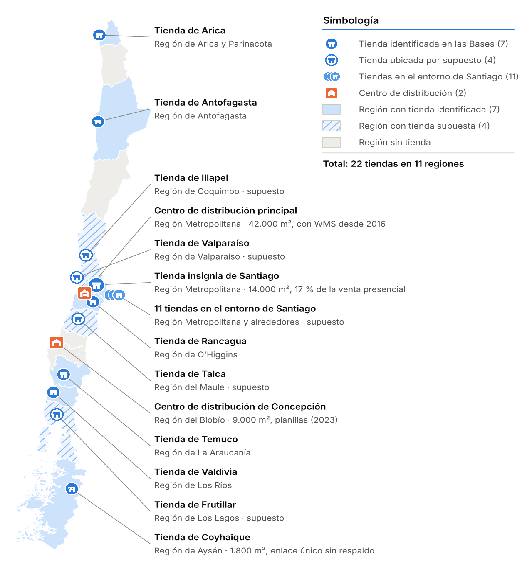
\includegraphics{figuras/figura-d96d9713821d-86e8742392.png}
\caption{Diagrama conceptual de solución e interacción de actores}
\end{figure}

Tabla 2.2:** Indicadores por promesa: valor actual, referencia y brecha.

\begin{longtable}[]{@{}
  >{\raggedright\arraybackslash}p{(\columnwidth - 8\tabcolsep) * \real{0.2000}}
  >{\raggedright\arraybackslash}p{(\columnwidth - 8\tabcolsep) * \real{0.2000}}
  >{\raggedright\arraybackslash}p{(\columnwidth - 8\tabcolsep) * \real{0.2000}}
  >{\raggedright\arraybackslash}p{(\columnwidth - 8\tabcolsep) * \real{0.2000}}
  >{\raggedright\arraybackslash}p{(\columnwidth - 8\tabcolsep) * \real{0.2000}}@{}}
\toprule\noalign{}
\begin{minipage}[b]{\linewidth}\raggedright
Promesa que busca cumplir ancoa
\end{minipage} & \begin{minipage}[b]{\linewidth}\raggedright
Indicador
\end{minipage} & \begin{minipage}[b]{\linewidth}\raggedright
Valor actual
\end{minipage} & \begin{minipage}[b]{\linewidth}\raggedright
Criterio de aceptación de Ancoa
\end{minipage} & \begin{minipage}[b]{\linewidth}\raggedright
Diferencia entre el valor actual y el criterio de aceptación
\end{minipage} \\
\midrule\noalign{}
\endhead
\bottomrule\noalign{}
\endlastfoot
\textbf{1. El producto existe} & Diferencias detectadas en conteo cíclico & 12,4 \% & \textless{} 2 \% & 6,2 veces \\
& Merma o pérdida desconocida sobre la venta & 1,9 \% & \textless{} 1 \% & 1,9 veces \\
& Pedidos en línea cancelados por falta de existencia, 2025 & 1,9 \% & \textless{} 0,3 \% & 6,3 veces \\
& Pedidos cancelados en el evento de junio de 2026 & 2,7 \% & 0 & Sin tolerancia \\
\textbf{2. El precio es el exhibido} & Productos con precio exhibido distinto del cobrado (muestra de 120) & 11 \% & Sin valor numérico & No calculable \\
\textbf{3. La entrega llega en la fecha} & Pedidos entregados en la fecha ofrecida & 81 \% & \textgreater{} 97 \% & 6,3 veces (19 \% frente a 3 \% fuera de plazo) \\
\textbf{4.Las condiciones del crédito son las informadas} & Tiempo de evaluación crediticia en el punto de venta & 40 s a 3 min & \textless{} 10 s & 4 a 18 veces \\
& Repactaciones sin evidencia recuperable del consentimiento & 1.240 & 0 & Sin tolerancia \\
& Conservación de las grabaciones de originación y repactación & 90 días & Plazo del crédito + 6 años & 24,3 veces o más \\
\end{longtable}

Como muestra la tabla, ninguna de las cuatro promesas alcanza la referencia definida y en tres de ellas, la compañía tampoco cuenta con un registro que le permita demostrar lo ocurrido.

\hypertarget{promesa-1-el-producto-existe}{%
\subsection{Promesa 1: El producto existe}\label{promesa-1-el-producto-existe}}

En cuanto a las

\hypertarget{promesa-2-el-precio-es-el-exhibido}{%
\subsubsection{Promesa 2: El precio es el exhibido}\label{promesa-2-el-precio-es-el-exhibido}}

En cuanto a las

\hypertarget{promesa-3-la-entrega-llega-en-la-fecha}{%
\subsubsection{Promesa 3: La entrega llega en la fecha}\label{promesa-3-la-entrega-llega-en-la-fecha}}

En cuanto a las

\hypertarget{promesa-4-las-condiciones-del-cruxe9dito-son-las-informadas-hola-samira-donde-estashola-samira-donde-estas}{%
\subsubsection{Promesa 4: Las condiciones del crédito son las informadas** HOLA SAMIRA DONDE ESTASHOLA SAMIRA DONDE ESTAS}\label{promesa-4-las-condiciones-del-cruxe9dito-son-las-informadas-hola-samira-donde-estashola-samira-donde-estas}}

En cuanto a las

\hypertarget{suxedntesis}{%
\subsubsection{Síntesis \ldots\ldots\ldots\ldots{}}\label{suxedntesis}}

En cuanto a las

\hypertarget{actores-y-grupos-de-interuxe9s}{%
\section{2.4 Actores y Grupos de Interés}\label{actores-y-grupos-de-interuxe9s}}

El problema de Ancoa S.A. involucra actores internos y externos pertenecientes a los dominios comercial, operacional, tecnológico y financiero. No todos estos actores enfrentan los problemas de la misma manera, algunos poseen la capacidad para condicionar decisiones, imponer restricciones o bloquear cambios, mientras otros se encuentran principalmente expuestos a las consecuencias de las inconsistencias de inventario, precios, pedidos y crédito.

Para este análisis, la influencia corresponde a la capacidad de un actor para condicionar decisiones, restricciones o procesos relevantes para Ancoa. El interés representa el grado en que ese actor se encuentra afectado por el problema o depende de que la compañía pueda cumplir y acreditar sus cuatro promesas operacionales: existencia del producto, precio exhibido, fecha de entrega y condiciones del crédito.

Las distintas áreas de Ancoa enfrentan el problema desde objetivos y responsabilidades diferentes. Mientras algunas buscan maximizar disponibilidad, velocidad de venta o aprovechamiento comercial de la información, otras deben resguardar exactitud operacional, trazabilidad y cumplimiento regulatorio. Estas diferencias generan tensiones que condicionan la operación y la toma de decisiones.

\hypertarget{actores-afectados-y-grupos-de-interuxe9s}{%
\subsection{Actores afectados y grupos de interés}\label{actores-afectados-y-grupos-de-interuxe9s}}

Los actores identificados se agrupan según la naturaleza de su participación y su capacidad para incidir en la operación de Ancoa. Esta agrupación permite distinguir a quienes intervienen directamente en las decisiones del negocio, a quienes ejecutan los procesos afectados y a los grupos externos cuya actuación condiciona el funcionamiento de la compañía. La Tabla 2.X sintetiza los principales grupos de interés y su nivel relativo de influencia e interés.

\begin{longtable}[]{@{}
  >{\raggedright\arraybackslash}p{(\columnwidth - 6\tabcolsep) * \real{0.2500}}
  >{\raggedright\arraybackslash}p{(\columnwidth - 6\tabcolsep) * \real{0.2500}}
  >{\raggedright\arraybackslash}p{(\columnwidth - 6\tabcolsep) * \real{0.2500}}
  >{\raggedright\arraybackslash}p{(\columnwidth - 6\tabcolsep) * \real{0.2500}}@{}}
\toprule\noalign{}
\begin{minipage}[b]{\linewidth}\raggedright
Grupo
\end{minipage} & \begin{minipage}[b]{\linewidth}\raggedright
Actores principales
\end{minipage} & \begin{minipage}[b]{\linewidth}\raggedright
Influencia
\end{minipage} & \begin{minipage}[b]{\linewidth}\raggedright
Interés
\end{minipage} \\
\midrule\noalign{}
\endhead
\bottomrule\noalign{}
\endlastfoot
Dirección y control & Directorio, Gerencia General, Contraloría & Alta & Alta \\
Propiedad & Grupo familiar controlador y fondos de inversión & Alta & Media \\
Negocios y operación & Comercial, Canales Digitales, Logística, Negocio Financiero & Alta & Alta \\
Soporte tecnológico y control operacional & TI, Prevención de Pérdidas & Alta & Alta \\
Operación de tienda & Jefaturas, vendedores, cajeros, reposición y bodega & Media & Alta \\
Clientes y terceros operacionales & Clientes, titulares de tarjeta, vendedores de marketplace, proveedores tecnológicos y logísticos & Baja -- media & Alta \\
Organismos externos & Autoridad financiera, autoridad de protección al consumidor y autoridad tributaria & Alta & Media -- alta \\
\end{longtable}

Fuente: elaboración propia.

La mayoría de actores con alta influencia e interés se concentran dentro de la misma organización. Esto se debe a la naturaleza transversal del problema, comercial administra surtido, precios y campañas, canales digitales utiliza la disponibilidad registrada para comprometer pedidos, logística depende de esa misma información para abastecer y despachar, el negocio financiero requiere agilidad en la atención y originación, contraloría debe resguardar la acreditación y separación entre ambos negocios, y TI sostiene el conjunto de plataformas e integraciones sobre las cuales operan estos procesos.

Los actores encargados de la operación de la tienda tienen una influencia menor sobre las decisiones corporativas, pero un interés elevado debido a su interacción diaria con los problemas. Ancoa cuenta con \textbf{3.820 vendedores de piso y cajeros}, con una rotación anual del 62 \%, además de personal de reposición, bodega y aproximadamente 1.100 repositores pertenecientes a proveedores externos que trabajan dentro de las salas de venta.

Los clientes, titulares de tarjetas, vendedores del marketplace y proveedores poseen una menor capacidad para influenciar las decisiones internas, pero experimentan directamente las consecuencias de las inconsistencias. Especialmente el cliente, el cual interactúa con la misma marca independiente de si su compra corresponde al canal presencial, digital, marketplace o al uso de la tarjeta propia, por lo que la fragmentación interna se vuelve visible cuando una promesa no puede cumplirse o acreditarse.

\hypertarget{matriz-influencia---interuxe9s}{%
\subsubsection{Matriz influencia - interés}\label{matriz-influencia---interuxe9s}}

La caracterización anterior permite ubicar a los principales actores y grupos de interés según dos variables, las cuales son, su capacidad para influir en las decisiones y procesos de Ancoa y el grado en que se encuentran afectados por el problema. Esta relación se representa en la Figura 2.X mediante cuatro cuadrantes que permiten diferenciar el nivel de atención requerido para cada grupo.

{[}{]}{[}image2{]}Fuente: elaboración propia

La mayor concentración se encuentra en el cuadrante de alta influencia y alto interés, en este se ubican el directorio y gerencia general, contraloría, comercial, canales digitales, logística, negocio financiero, TI, prevención de pérdidas, y las principales autoridades fiscalizadoras. Estos actores poseen la capacidad para condicionar las decisiones relevantes, y al mismo tiempo, están directamente vinculados con las consecuencias operacionales, comerciales y regulatorias del problema, razón por la cual requieren un involucramiento cercano en el proceso del proyecto.

En el cuadrante de alta influencia y menor interés se encuentran el grupo familiar controlador, los fondos de inversión y la autoridad tributaria. Su participación en la operación cotidiana es menor, pero mantienen capacidad para condicionar decisiones corporativas o establecer obligaciones que Ancoa debe cumplir. En consecuencia, requieren mantenerse satisfechos y ser consultados en aquellas materias que afecten sus ámbitos de responsabilidad.

Los actores de menor influencia y alto interés corresponden principalmente a quienes experimentan directamente los efectos de las deficiencias actuales: jefaturas de tienda, vendedores y cajeros, personal de reposición y bodega, clientes, titulares de tarjeta, vendedores del marketplace y proveedores tecnológicos y logísticos. Aunque disponen de menor capacidad para determinar las decisiones corporativas, su participación resulta relevante porque ejecutan los procesos afectados o reciben directamente sus consecuencias. Estos grupos deben mantenerse informados y considerados en el levantamiento de necesidades operacionales.

Finalmente, los administradores de centros comerciales y los repositores externos se ubican en el cuadrante de menor influencia y menor interés relativo. Su participación se concentra en ámbitos específicos de la operación y poseen una capacidad limitada para modificar las decisiones generales de Ancoa, por lo que requieren principalmente seguimiento.

Esta distribución evidencia que la gestión de los grupos de interés no puede concentrarse únicamente en los niveles directivos. Los actores con mayor influencia determinan restricciones y decisiones relevantes, mientras que una parte importante de quienes poseen alto interés corresponde a usuarios, clientes y terceros que interactúan diariamente con los procesos afectados. Esta diferencia entre capacidad de decisión y exposición al problema permite anticipar los puntos donde será necesaria una mayor coordinación entre los distintos grupos durante el proyecto.

\hypertarget{tensiones-entre-interesados.}{%
\subsubsection{Tensiones entre interesados.}\label{tensiones-entre-interesados.}}

Las tensiones identificadas surgen de objetivos, incentivos y responsabilidades que no siempre coinciden. Algunas son desacuerdos expresos entre actores; otras son desajustes de coordinación entre quienes prometen, ejecutan y reciben un servicio. Su identificación permite comprender el problema sin anticipar el diseño de la solución.

Una de las tensiones más explícitas se presenta entre el Negocio Financiero y Contraloría. Álvaro Peña necesita que la evaluación crediticia se resuelva en segundos para evitar la pérdida de ventas y favorecer el uso de la tarjeta propia. Cecilia Bordalí exige que la información precontractual completa se entregue antes de la aceptación y que quede evidencia recuperable de lo informado y consentido. Ambos reconocen la tensión entre rapidez comercial y cumplimiento, aunque Álvaro también reconoce la necesidad de acreditar las operaciones de la filial fiscalizada

El conflicto también afecta a los vendedores de piso, cuyos incentivos económicos dependen de cerrar ventas y promover la tarjeta propia. Jonathan Millán explica que su comisión mejora cuando el cliente paga con tarjeta y advierte que dejaría de ofrecer si el proceso se vuelve más largo. Además, reconoce que la presión de atender filas lo lleva a entregar el documento precontractual y comunicar sólo sus aspectos principales. Cecilia señala que la capacitación, por sí sola, no resuelve esta situación, porque el incentivo a cerrar rápidamente permanece.

Entre Canales Digitales y Logística existe una tensión relacionada con la cantidad de existencia que puede publicarse sin comprometer productos que la compañía no podrá entregar. Nicolás Errázuriz necesita mantener una oferta comercial competitiva, pero reconoce que depende de un inventario impreciso y de un descuento de seguridad fijo. Fernanda Quilaqueo destaca que la reposición y el cumplimiento de pedidos dependen de la calidad de ese registro. Publicar menos reduce el riesgo de cancelaciones, pero también puede reducir las ventas.

La Gerencia Comercial y la operación de tienda enfrentan ritmos distintos para gestionar los precios. Rodrigo Sanhueza considera necesario modificarlos varias veces al día para responder a la competencia, mientras Marisol Tapia explica que las etiquetas físicas se reemplazan de noche y que el personal no siempre alcanza a completar todos los cambios. La decisión comercial se aplica en cajas y en el canal digital antes de reflejarse en la sala, generando diferencias entre el precio exhibido y el cobrado

El despacho desde tienda genera otra tensión entre el canal digital y las jefaturas y vendedores de los locales. Para el canal digital, utilizar unidades de las tiendas permite acercar el producto al cliente. Sin embargo, la tienda debe destinar personal a preparar pedidos y entregar unidades que podrían venderse presencialmente, sin que el vendedor reciba la comisión correspondiente. Marisol señala que esta práctica perjudica los resultados de su tienda, Jonathan manifiesta su molestia por perder unidades que tenía comprometidas con clientes y Fernanda advierte que la tienda no fue diseñada para operar como bodega y preparar pedidos en línea.

Marketing y Contraloría presentan una tensión respecto del aprovechamiento comercial de los datos financieros. Según la entrevista de Cecilia, Marketing busca utilizar el comportamiento de pago para segmentar ofertas del retail. Contraloría advierte que esa información fue obtenida en un negocio regulado y que su utilización requiere definir la finalidad, la base que autoriza el cruce y los controles aplicables. Su posición no establece una prohibición absoluta de compartir información, sino que cuestiona hacerlo sin reglas documentadas y auditables.

También existe una diferencia entre las prioridades del comité y la urgencia del Negocio Financiero. El comité prefiere atender primero la exactitud del inventario y los precios, dejando el negocio financiero para después. Álvaro objeta esa secuencia porque el plan de remediación y el soporte de la plataforma crediticia vencen en 2029, y la migración de una cartera viva requiere preparación y convivencia suficientes.

Estas tensiones muestran que el problema no se explica únicamente por limitaciones tecnológicas. También intervienen incentivos comerciales, capacidad de ejecución, distribución de responsabilidades y restricciones del negocio fiscalizado. Comprenderlas es necesario para comprender las condiciones que debe considerar posteriormente la propuesta para cumplir y acreditar las cuatro promesas.

\hypertarget{resumen-de-requerimientos-supuestos-exclusiones-y-restricciones}{%
\section{2.5 Resumen de Requerimientos, Supuestos, Exclusiones y Restricciones}\label{resumen-de-requerimientos-supuestos-exclusiones-y-restricciones}}

Esta sección resume y analiza lo que el cliente requiere, los supuestos que el equipo declara para interpretar la información disponible, con su respectivo fundamento, y las exclusiones y restricciones que impone el caso. Su propósito es dejar explícito, antes de describir la solución, qué se debe cumplir, que se da por supuesto y lo que queda fuera de la propuesta.

El detalle de cada elemento con su identificador individual, se encuentra en el archivo de anexos correspondiente a este subdocumento, contiene el listado de requerimientos, el listado de supuestos, exclusiones y restricciones y otros listados de apoyo.

\hypertarget{resumen-de-requerimientos}{%
\subsection{Resumen de requerimientos}\label{resumen-de-requerimientos}}

Los requerimientos se obtuvieron en base a lo estipulado por el cliente, de modo que exprese una sola condición verificable. Se clasificaron en tres tipos, 223 requerimientos funcionales (RF), que describen lo que el sistema debe hacer, 75 requerimientos no funcionales (RFN), que fijan un umbral medible y su método de verificación, que corresponden a compromisos de la oferta y no a funciones del sistema por lo que no admiten caso de prueba d software.

La Tabla 2.1 resume su distribución por categoría.

Tabla 2.1:** Requerimientos del CLIENTE por tipo y categoría.

\textbf{Tabla --- bloque 1 de 3.}

\begin{longtable}[]{@{}
  >{\raggedright\arraybackslash}p{(\columnwidth - 4\tabcolsep) * \real{0.3333}}
  >{\raggedright\arraybackslash}p{(\columnwidth - 4\tabcolsep) * \real{0.3333}}
  >{\raggedright\arraybackslash}p{(\columnwidth - 4\tabcolsep) * \real{0.3333}}@{}}
\toprule\noalign{}
\begin{minipage}[b]{\linewidth}\raggedright
Tipo y categoría
\end{minipage} & \begin{minipage}[b]{\linewidth}\raggedright
N.º
\end{minipage} & \begin{minipage}[b]{\linewidth}\raggedright
Síntesis de lo que exige el CLIENTE
\end{minipage} \\
\midrule\noalign{}
\endhead
\bottomrule\noalign{}
\endlastfoot
RF Pedidos y cumplimiento & 47 & Promesa de entrega confiable, elección del punto de despacho por costo total de servir, y retiro o despacho desde tienda. \\
RF Inventario y disponibilidad & 38 & Cálculo centralizado del disponible para vender, conteo cíclico por clasificación ABC y clasificación obligatoria de la merma. \\
RF Crédito y cobranza & 28 & Evaluación y cupo en el punto de venta, evidencia del consentimiento y de la información precontractual, y migración de la cartera. \\
RF -- Marketplace & 25 & Reglas de desempeño y sanciones para los vendedores externos, gestión de catálogo y devoluciones. \\
RF -- Operación de tienda & 20 & Continuidad en modo desconectado: venta, cobro, promociones y documento de venta en contingencia. \\
RF -- Precios y etiquetado & 16 & Coherencia entre el precio exhibido y el cobrado, y evidencia del precio publicado. \\
RF -- Seguridad y accesos & 14 & Credenciales individuales, sin acceso anónimo ni credenciales compartidas. \\
RF -- Gobernanza de datos & 12 & Separación de datos entre retail y filial financiera, finalidad declarada e inventario de interfaces. \\
RF -- Devoluciones y garantía legal & 12 & Atención íntegra en el mesón, sin derivar al cliente, y decisión de aptitud antes de reingresar una unidad al stock. \\
RF -- Evento de alta concurrencia & 10 & Degradación controlada de servicios y bloqueo de despliegues en las cinco ventanas de congelamiento. \\
\end{longtable}

\textbf{Tabla --- bloque 2 de 3.}

\begin{longtable}[]{@{}
  >{\raggedright\arraybackslash}p{(\columnwidth - 4\tabcolsep) * \real{0.3333}}
  >{\raggedright\arraybackslash}p{(\columnwidth - 4\tabcolsep) * \real{0.3333}}
  >{\raggedright\arraybackslash}p{(\columnwidth - 4\tabcolsep) * \real{0.3333}}@{}}
\toprule\noalign{}
\begin{minipage}[b]{\linewidth}\raggedright
Tipo y categoría
\end{minipage} & \begin{minipage}[b]{\linewidth}\raggedright
N.º
\end{minipage} & \begin{minipage}[b]{\linewidth}\raggedright
Síntesis de lo que exige el CLIENTE
\end{minipage} \\
\midrule\noalign{}
\endhead
\bottomrule\noalign{}
\endlastfoot
RF -- Ventas en tienda & 1 & Prioridad de la venta física sobre una reserva digital temporal. \\
\textbf{Subtotal RF} & \textbf{223} & \\
RNF -- Seguridad & 16 & Arquitectura segura, segmentación de red en las 22 tiendas, separación acreditada de la filial, tokenización de medios de pago y DevSecOps. \\
RNF -- Desempeño y capacidad & 15 & Tiempos de respuesta (evaluación crediticia ≤ 8 s, confirmación de pedido ≤ 3 s, propagación de precios ≤ 5 min) y soporte del peak del evento anual. \\
RNF -- Cumplimiento y auditabilidad & 13 & Plazos de conservación de la evidencia, base de licitud y registro de actividades de tratamiento de datos. \\
RNF -- Disponibilidad y recuperabilidad & 11 & Operación sin enlace externo (≥ 8 h en tienda), recuperación ante desastres (RTO ≤ 4 h; RPO ≤ 15 min). \\
RNF -- Operabilidad e interoperabilidad & 10 & Notificaciones y avisos oportunos al cliente, y estándares de intercambio con proveedores. \\
RNF -- Migración, portabilidad y escalabilidad & 4 & Migración de 620.000 clientes con saldo sin pérdida, interrupción ni divergencias; apertura de tiendas por parametrización. \\
RNF -- Efectividad de negocio & 3 & Metas sobre la línea base: cancelación \textless{} 0,3 \%, cumplimiento de entrega ≥ 97 \% y diferencia de inventario \textless{} 2 \%. \\
RNF -- Usabilidad & 2 & Operación con capacitación mínima y lenguaje claro en las comunicaciones del crédito. \\
\end{longtable}

\textbf{Tabla --- bloque 3 de 3.}

\begin{longtable}[]{@{}
  >{\raggedright\arraybackslash}p{(\columnwidth - 4\tabcolsep) * \real{0.3333}}
  >{\raggedright\arraybackslash}p{(\columnwidth - 4\tabcolsep) * \real{0.3333}}
  >{\raggedright\arraybackslash}p{(\columnwidth - 4\tabcolsep) * \real{0.3333}}@{}}
\toprule\noalign{}
\begin{minipage}[b]{\linewidth}\raggedright
Tipo y categoría
\end{minipage} & \begin{minipage}[b]{\linewidth}\raggedright
N.º
\end{minipage} & \begin{minipage}[b]{\linewidth}\raggedright
Síntesis de lo que exige el CLIENTE
\end{minipage} \\
\midrule\noalign{}
\endhead
\bottomrule\noalign{}
\endlastfoot
RNF -- Consistencia de datos & 1 & Mismo estado del pedido en todos los canales de consulta. \\
\textbf{Subtotal RNF} & \textbf{75} & \\
OP -- Obligaciones del proponente & 9 & Alternativa de etiquetas electrónicas, dispositivos móviles por tienda y análisis de hacer o comprar del CD de Concepción. \\
\textbf{Total} & \textbf{307} & \\
\end{longtable}

\hypertarget{fuente-elaboraciuxf3n-propia-a-partir-de-empresa-subdocumento2-anexos-anexos-a.1-a-a.3.}{%
\subsubsection{Fuente: Elaboración propia a partir de EMPRESA-Subdocumento2-Anexos, Anexos A.1 a A.3.}\label{fuente-elaboraciuxf3n-propia-a-partir-de-empresa-subdocumento2-anexos-anexos-a.1-a-a.3.}}

La distribución muestra que el 62 \% de los requerimientos funcionales (138 de 223) se concentra en cuatro categorías: pedidos y cumplimiento, inventario y disponibilidad, crédito y cobranza, y marketplace. Esta concentración es coherente con el diagnóstico, porque esas categorías sostienen directamente tres de las cuatro promesas de Ancoa: que el producto existe, que la entrega llegará en la fecha informada y que las condiciones del crédito son aceptadas. La cuarta promesa, que el precio cobrado coincida con el exhibido, se aborda en la categoría de precios y etiquetado, que tiene menos requerimientos, pero un alto impacto regulatorio.

Los requerimientos no funcionales, por su parte, convierten el problema dimensionado en metas verificables. Tres de ellos fijan la mejora esperada respecto de la línea base: reducir la cancelación por falta de existencia a menos de 0,3 \% anual, elevar el cumplimiento de la fecha de entrega desde 81 \% a 97 \% o más, y bajar la diferencia de inventario por categoría desde 12,4 \% a menos de 2 \%. Otros tres exigen que la migración de los 620.000 clientes con saldo se complete sin pérdida de datos, sin interrupción del cobro y sin divergencias de saldo antes de 2029. Las obligaciones del proponente, en cambio, no describen funciones del sistema, sino entregables de la oferta, como el análisis de hacer o comprar del CD de Concepción.

A estos requerimientos se suman los 374 requisitos técnicos (RT) de las Bases. La relación entre cada requerimiento, el componente que lo satisface y la sección de la propuesta donde se desarrolla se presenta en la matriz de cumplimiento y trazabilidad del Anexo A.5.2.

\hypertarget{resumen-de-supuestos}{%
\subsubsection{Resumen de supuestos}\label{resumen-de-supuestos}}

Cuando las Bases describen un problema, pero no definen la regla con la que debe resolverse, el equipo declara un supuesto. Se declararon 25 supuestos (SUP-01 a SUP-25), cada uno con su fundamento en los datos del caso o en la normativa aplicable. Se agrupan en seis temas:

● \textbf{Inventario y disponibilidad (SUP-01, SUP-12, SUP-17, SUP-18 y SUP-20):} el disponible para vender se calcula de forma centralizada con un colchón de seguridad dinámico por categoría y tienda, las reservas del carro digital expiran, todo ajuste de inventario se clasifica según su causa y el CD de Concepción queda fuera del disponible mientras opere con planillas manuales.

● \textbf{Precios (SUP-08 a SUP-10):} ante una discrepancia prevalece el precio exhibido más bajo, el precio nuevo se activa en caja solo cuando se confirma el cambio de etiqueta y el historial de precios publicados se conserva de forma inalterable.

● \textbf{Pedidos y logística (SUP-11, SUP-13, SUP-14 y SUP-22):} ante un quiebre se ofrece sustitución, compra a terceros o entrega compensada antes de cobrar; el origen del despacho se elige por costo total de servir; la comisión se atribuye a la tienda que abastece el pedido; y el producto devuelto por retracto se inspecciona antes de reingresar al stock.

● \textbf{Marketplace y postventa (SUP-15, SUP-16 y SUP-21):} las garantías y devoluciones se resuelven en el mesón sin derivar al cliente, y los 310 vendedores externos operan con reglas de desempeño y sanciones automatizadas.

● \textbf{Crédito y datos personales (SUP-03 a SUP-07 y SUP-25):} identidad del cliente en dos capas, frontera de datos entre retail y filial cerrada por defecto, evidencia digital inalterable del consentimiento y de la hoja resumen, venta con crédito en modo desconectado contra un cupo preaprobado, y migración de la cartera por etapas con conciliación diaria y reversión.

● \textbf{Tecnología y personas (SUP-02, SUP-19, SUP-23 y SUP-24):} transición gradual sin reemplazo «Big Bang», con el ERP como único emisor tributario; degradación escalonada en eventos de alta demanda; y accesos individuales con altas y bajas automáticas para el personal propio, temporal y externo.

En conjunto, los supuestos comparten un mismo criterio: tratar los registros actuales como imperfectos y exigir evidencia verificable de cada promesa. Los más sensibles para la propuesta son SUP-02, SUP-04 y SUP-25, porque condicionan la estrategia de transición, la separación entre ambos negocios y la migración de la cartera financiera; si alguno de ellos no se confirma, cambia el plan de implantación. El listado completo, con el enunciado y el fundamento de cada supuesto, se encuentra en el Anexo A.4.1.

\hypertarget{resumen-de-exclusiones}{%
\subsubsection{Resumen de exclusiones}\label{resumen-de-exclusiones}}

Las exclusiones delimitan lo que la propuesta no asume, ya sea porque las Bases lo dejan fuera del alcance o porque la información disponible no permite sostenerlo. Se identificaron ocho exclusiones (EXC-01 a EXC-08), de dos tipos:

● \textbf{De alcance (EXC-01 a EXC-06):} la adquisición de etiquetas electrónicas, que se especifica y costea por separado sin incluir su compra; el CD de Concepción como origen de la promesa de entrega mientras no acredite su sistema de gestión de almacenes; el reemplazo del ERP heredado como emisor tributario; la sustitución simultánea de las nueve plataformas actuales; la gestión laboral y la capacitación de los repositores externos; y cualquier flujo que derive al cliente a terceros en garantías o devoluciones.

● \textbf{Del análisis (EXC-07 y EXC-08):} no se proyecta el 11 \% de discrepancia de precios más allá de la muestra fiscalizada, ni se descompone la merma histórica entre pérdida física y error de registro, porque las Bases no entregan información suficiente para hacerlo.

Declarar estas exclusiones evita comprometer resultados que dependen de decisiones del CLIENTE o de información que hoy no existe. El detalle y el origen de cada exclusión se presentan en el Anexo A.4.2.

\hypertarget{resumen-de-restricciones}{%
\subsubsection{Resumen de restricciones}\label{resumen-de-restricciones}}

Las restricciones son condiciones del caso que la solución no puede modificar y dentro de las cuales debe operar. Se identificaron 15 restricciones (RES-01 a RES-15), que la Tabla 2.2 agrupa por tipo junto con su efecto sobre la propuesta.

Tabla 2.2:** Síntesis de restricciones por tipo.

\begin{longtable}[]{@{}
  >{\raggedright\arraybackslash}p{(\columnwidth - 4\tabcolsep) * \real{0.3333}}
  >{\raggedright\arraybackslash}p{(\columnwidth - 4\tabcolsep) * \real{0.3333}}
  >{\raggedright\arraybackslash}p{(\columnwidth - 4\tabcolsep) * \real{0.3333}}@{}}
\toprule\noalign{}
\begin{minipage}[b]{\linewidth}\raggedright
Tipo
\end{minipage} & \begin{minipage}[b]{\linewidth}\raggedright
Restricciones principales
\end{minipage} & \begin{minipage}[b]{\linewidth}\raggedright
Efecto en la propuesta
\end{minipage} \\
\midrule\noalign{}
\endhead
\bottomrule\noalign{}
\endlastfoot
Regulatoria (RES-01 a RES-05) & Ley N.º 19.496; Decreto N.º 6 de 2021; Ley N.º 18.010 y fiscalización de la CMF; Ley N.º 21.719, vigente desde el 1 de diciembre de 2026; plazos de conservación de la evidencia. & Cada operación debe dejar evidencia verificable y respetar el régimen del negocio al que pertenece. El cruce de datos entre retail y filial queda cerrado por defecto. \\
Temporal (RES-06 a RES-08) & Fin del soporte de la plataforma de originación y cobranza, y último hito del plan de remediación, en 2029; cinco ventanas anuales de congelamiento; eventos comerciales con fechas fijadas externamente. & El plan de implantación debe calzar entre las ventanas de congelamiento y terminar la migración financiera antes de 2029. \\
Tecnológica y de infraestructura (RES-09 a RES-11) & Nueve plataformas y catorce interfaces punto a punto sin mapa completo; infraestructura compartida con la filial; 14 tiendas dependientes del enlace del centro comercial y 13 sin segmentación de red. & La transición debe ser gradual, con operación desconectada en tienda y separación acreditada de la filial. \\
Migración (RES-12) & 620.000 clientes con saldo que deben migrarse sin pérdida de datos, interrupción del cobro ni divergencias de saldo. & Migración por etapas, con coexistencia de plataformas y conciliación diaria de saldos. \\
Humana y organizacional (RES-13 a RES-15) & 3.820 vendedores y cajeros con rotación anual del 62 \%; 1.900 contrataciones de temporada; 640 terminales compartidos; 1.100 repositores externos; 46 profesionales de TI en el CLIENTE. & Interfaces operables con capacitación mínima, traspaso rápido de sesión en terminales compartidos y una carga de cambio acotada para el equipo del CLIENTE. \\
\end{longtable}

\hypertarget{fuente-elaboraciuxf3n-propia-a-partir-de-empresa-subdocumento2-anexos-anexo-a.4.3.}{%
\subsubsection{Fuente: Elaboración propia a partir de EMPRESA-Subdocumento2-Anexos, Anexo A.4.3.}\label{fuente-elaboraciuxf3n-propia-a-partir-de-empresa-subdocumento2-anexos-anexo-a.4.3.}}

El análisis de las restricciones muestra que el principal límite del proyecto no es tecnológico, sino regulatorio y temporal: la solución debe separar dos negocios que comparten cliente e infraestructura y, al mismo tiempo, migrar la cartera financiera antes de 2029 sin intervenir la operación durante las ventanas de congelamiento. El detalle de cada restricción y su origen se encuentra en el Anexo A.4.3.

\hypertarget{otros-listados}{%
\subsubsection{Otros listados}\label{otros-listados}}

Como apoyo, el Anexo A.5 incluye dos listados adicionales: los indicadores con su línea base y la meta comprometida (Anexo A.5.1), que conectan el dimensionamiento de la sección 2.3 con los requerimientos no funcionales, y la matriz de cumplimiento y trazabilidad (Anexo A.5.2), que relaciona cada requerimiento con el componente que lo satisface y la sección de la propuesta donde se desarrolla.

\ossFinalPage

\end{document}
